\documentclass{article}
\usepackage{CJKutf8}
\usepackage{indentfirst}
\usepackage{graphics}
\usepackage{epsfig}
\usepackage{graphicx}
\usepackage{amsmath}
\usepackage{amssymb}
\usepackage{listings}
\usepackage{color}
\usepackage{pgffor}
\usepackage[toc,page]{appendix}
\definecolor{dkgreen}{rgb}{0,0.6,0}
\definecolor{gray}{rgb}{0.5,0.5,0.5}
\definecolor{mauve}{rgb}{0.58,0,0.82}

\lstset{frame=tb,
	language=C,
	aboveskip=3mm,
	belowskip=3mm,
	showstringspaces=false,
	columns=flexible,
	basicstyle={\small\ttfamily},
	numbers=none,
	numberstyle=\tiny\color{gray},
	keywordstyle=\color{blue},
	commentstyle=\color{dkgreen},
	stringstyle=\color{mauve},
	breaklines=true,
	breakatwhitespace=true,
	tabsize=3
}
\setlength{\parindent}{2em}
\renewcommand{\contentsname}{目录}
\renewcommand{\listfigurename}{插图目录}
\renewcommand{\listtablename}{表格目录}
\renewcommand{\refname}{参考文献}
\renewcommand{\abstractname}{摘要}
\renewcommand{\indexname}{索引}
\renewcommand{\tablename}{表}
\renewcommand{\figurename}{图}
\renewcommand{\appendixname}{附录}
%opening
\date{2016年11月}
\title{词法分析实验报告}
\author{何宜晖\\计算机46\\2140504137\\电信学院\\heyihui@stu.xjtu.edu.cn}

\begin{document}
\begin{CJK}{UTF8}{gkai}
%gkai gbsn
\begin{figure}
\centering
\includegraphics[width=0.6\linewidth]{/home/eli/Pictures/xjtu}
\end{figure}


\maketitle
\clearpage
\section{实验目的}
\begin{enumerate}
	\item 强化对系统软件综合工程实现能力的训练
	\item 加强对词法分析原理、方法和基本实现技术的理解
\end{enumerate}

\section{实验内容}
用C语言或者其他的高级语言作为宿主语言完成C1语言的词法分析器的设计和实现。

\section{实验要求}
\begin{enumerate}
\item 编写C0语言的词法分析器的源程序并调试通过。其中词法分析程序既可以自己手动去完成,也可以利用LEX自动生成。
\item 通过测试程序的验收; 
\item 实验报告按照提供的模板填写 
\end{enumerate}

\section{功能描述}
该程序要实现的是一个读程序的过程,从输入的源程序中,识别出各种类型的单词(基本保留字、标识符、常数、运算符、分隔符)。输出并打印各个单词的类型以及本身.\cite{chen2000}\cite{appel2004modern}\cite{louden2000}\cite{appel2006}.
我编写了几个简单的c0语言程序,解析结果在附录\ref{append}中

类型名按照实验指导书定义,部分未出现的,参照 ANSI C \cite{ansic}

分析部分,可以开启yylineao,用于打开自动记录行号\verb|%option yylineao|。
匹配到的词可以用\verb|yytext|直接获取。

主程序部分,\verb|yyin|将读取到的文件传送给lex。 \verb|yylex()| 则开始词法分析,每个匹配到的词,都会执行后面动作。\cite{levine1992lex}\cite{lesk1975lex}
\subsection{注释的跳过}\label{sec:com}
读到\verb|\\|我们就吃掉整行。
读到\verb|\*|我们进入注释程序\verb|comment()|. 一直读取,直到读到\verb|*/|为止,否则报错。

\section{程序结构描述}
程序使用lex编写,按指导书给出的状态转换图进行正则匹配,状态转移图如图\ref{fig:state}所示。

程序中设计了一个关键的打印函数 printToken, 该函数输入为当前识别的类型,输出为打印当前的行号,字符,以及类型。另一个函数是comment函数,用来判断当前注释进行的状态,如果注释出错,则需要报错,在章节\ref{sec:com}中已经详细解释了。另外则是主函数main,用于读取程序,启动yylex()程序解析。
\begin{figure}[!h]
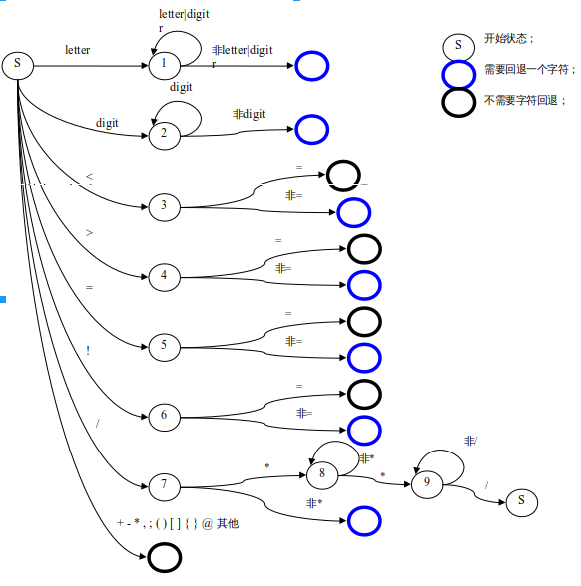
\includegraphics[width=\linewidth]{lex}
\caption{状态转换图}
\label{fig:state}
\end{figure}
\lstinputlisting[language=c]{../c-compiler/q1.l}

\section{实验总结}
\begin{enumerate}
\item 你在编程过程中花时多少?我大概花了一个晚上。
\item  多少时间在纸上设计?花了半小时在纸上设计。
\item  多少时间上机输入和调试?3个小时左右。
\item  多少时间在思考问题?一个小时左右。
\item  遇到了哪些难题,你是怎么克服的? 实验中还是遇到了很多难题。首先是如何使用lex,经过仔细阅读参考书目lex\&yacc\ref{levine1992lex}, 让我了解了lex的基本用法。还有就是如何显示行号,如何获得当前的字符,我通过上网搜索了解到可以使用yylineao,yytext。以及如何解决有注释的问题,虽然实验指导书没有给出,我还是在参考书目中感悟到了解决方法\ref{levine1992lex}
\item  你对你的程序的评价?我的程序使用lex编写,token定义模仿标准的ANIS C。自己比较满意。
\item  你的收获有哪些?这次实验学会了使用lex,为后面利用yacc进行语法分析打下了坚实的基础。
\end{enumerate}

{\small
	\bibliographystyle{ieee}
	\bibliography{he16yacc}
}
\clearpage

\appendix
\section{样例代码与输出}\label{append}

\foreach \n in {orig.c,simple.c,test.c,test2.c,testlex.c,testparser.c}{
	 $c_0$ 语言文件 \n
	\lstinputlisting[language=c]{../c-compiler/test/\n}
	$c_0$ 语言文件 \n 的输出
	\lstinputlisting[language=xml]{../c-compiler/test/\n.lex.xml}
}

\end{CJK}
\end{document}
